\documentclass[a4paper]{article}
\usepackage[slovene]{babel}
\usepackage[utf8]{inputenc}
\usepackage[T1]{fontenc}
\usepackage{graphicx}
\usepackage{marvosym}
\usepackage{amssymb,amsmath}
\title{Upravljanje maloprodajnega prostora}
\author{Leon Horvat, Jernej Banevec \\ Finančni praktikum \\ Finančna matematika, Fakulteta za matematiko in fiziko}
\date{2017}


\begin{document}
\title{%
  Upravljanje omejenega maloprodajnega prostora za osnovne izdelke \\
  \large Kratko poročilo \\}

\author{Jernej Banevec, Leon Horvat}

\maketitle

\pagebreak

\section{Uvod}


Maloprodajne trgovine imajo veliko izbiro izdelkov, ki jih lahko vključijo v svojo ponudbo, hkrati pa so omejeni s prostorom v posamezni trgovini. Lahko se odločijo, da bodo imeli več različnih produktov z manjšimi zalogami na policah in posledično pogostejšim polnjenjem polic ali pa manj produktov z večjimi zalogami. Nepravilna izbira lahko vodi v nižji dobiček. Trgovci se morajo pri upravljanju maloprodajnega prostora odločiti, katere izdelke vključiti v svojo ponudbo ter optimizirati velikost zalog na policah in urnik njihovega polnjenja. Ti dve odločitvi sta tesno povezani, zato jih moramo obravnavati sočasno. 


Pri analizi problema se bova osredotočila na trgovine, ki imajo v svojo ponudbo vključene izdelke z dolgo življenjsko dobo in stabilnim povpraševanjem. 

Med trgovci sta se oblikovali dve strategiji za razporeditev izdelkov: strategija dodeljenega prostora in strategija skupnega prostora. Pri strategiji dodeljenega prostora ima vsak izdelek svoj točno določen prostor, pri strategiji skupnega prostora pa je dovoljeno deljenje prostora. Na primer trgovci lahko določenemu izdelku namenijo 20 centimetrov širine police, lahko pa neki skupini izdelkov namenijo prostor, v katerem je razporeditev odvisna od zaloge posameznega izdelka na polici; če ravno dopolnemo zalogo enega izdelka, mora biti ostalih manj, da je na polici dovolj prostora. Če je prostor dodeljen izdelku, je upravljanje urnika polnjenja polic manj zahtevno kot pri strategiji skupnega prostora. Pri slednji morajo biti trgovci na to bolj pozorni, ker lahko v primeru istočasnega polnjenja polic s temi izdelki zmanjka prostora. 

\vspace{4 mm}

\begin{figure}[h]
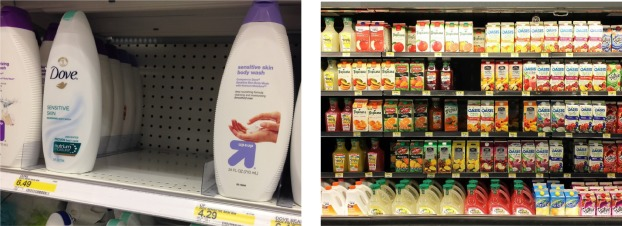
\includegraphics [scale = 0.8]{zgled-strategij}
\caption{Primer strategije dodeljenega prostora in strategije skupnega prostora}
\centering
\end{figure}

Za zgled vzemimo 2 izdelka X in Y, ki imata oba enako velikost 1. Namenimo jima 10 enot prostora. Zalogi obeh se obnavljata na 6 dni. Če obnovimo obe zalogi hkrati, torej prvi dan, prostora na polici ni dovolj glede na povpraševanje izdelka. Če pa zalogo drugega obnovimo prvi dan, prvega pa četrti dan, potrebujemo manj prostora in 10 enot zadostuje povpraševanju obeh izdelkov. Opazimo, da pri uporabi strategije skupnega prostora porabimo manj prostora, vendar je potrebna koordinacija polnjenja zalog izdelkov, ki si delijo prostor.

\begin{figure}[ht]
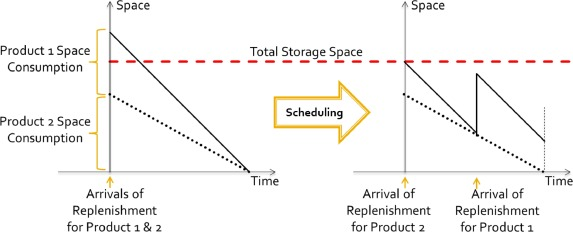
\includegraphics [scale = 0.8]{primerjava-strategij}
\caption{Poraba prostora strategij}
\end{figure}



\section{Modeliranje problema}

Upravljanje maloprodajnega prostora je formulirano kot nelinearen mešan celoštevilski program. Naj bo $\mathcal{P}= \{1, 2, ..., M\}$ indeksna množica možnih produktov. Predpostavimo, da imamo konstantno količino varnostne zaloge, ki je potrebna zaradi nihanja povpraševanja. Ta količina je lahko izračunana iz variacije povpraševanja in zahtevane ravni storitev, ki bo v našem primeru blizu 100 odstotkov, to pomeni da bo zelo majhna verjetnost, da katerega koli produkta zmanjka. Zaradi visoke zahtevane ravni storitev bomo v modelu upoštevali samo učinek substitucije izdelkov, ki jih nimamo v ponudbi, učinek substitucije razprodanih izdelkov pa zanemarimo. Predpostavimo tudi, da je povpraševanje eksogeno. Za vsak izdelek iz množice  $\mathcal{P}$, ki ni vključen v ponudbo, se del njegovega povpraševanja prenese na izdelke, ki so v ponudbo vključeni. Ta del povpraševanja zaradi substitucije manjkajočega izdelka je konstanten in neodvisen od ponudbe ostalih izdelkov. 

\vspace{3 mm}
Definirajmo:
\begin{itemize}
\item parametre:
\begin{itemize}
\item $ d_i $: prvotna stopnja povpraševanja po izdelku $i$,
\item $ w_{ij}$: delež povpraševanja izdelka $j$ prenesenega na izdelek $i$, če $j$-tega izdelka ni v ponudbi; $w_{ii} = 1$,
\item $ v_i $: dobiček pri $i$-tem izdelku,
\item $ h_i $: strošek hranjenja izdelka $i$ na polici,
\item $ k_i $: cena polnjenja izdelka $i$, 
\item $ \theta_i $: koeficient količine varnostne zaloge izdelka $i$.
\end{itemize}

\item odločitvene spremenljivke:
\begin{itemize}
\item $ y_i $: indikator, ki nam pove, ali je izdelek $i$ vključen v ponudbo,
\item $ Q_i $: število naročenih izdelkov $i$.
\end{itemize}

\item pomožne spremenljivke:
\begin{itemize}
\item $ x_{ij} $: indikator substitucije iz izdelka $j$ na izdelek $i$; $x_{ij} = y_i (1-y_j)$, če $j \ne i$ in $x_{ij} = y_i$, če  $j = i$,
\item $ s_i $: končna efektivna stopnja povpraševanja po $i$-tem izdelku; $s_i = y_i (d_i + \sum_{j \ne i} w_{ij} d_j (1-y_j)) = \sum_j  w_{ij} d_j x_{ij}.$
\end{itemize} 
\end{itemize}

<<<<<<< HEAD
 Pri problemu bomo predpostavili neodvisno polnjenje polic, torej da  ima vsak izdelek svoj strošek polnjenja. Lahko bi uporabili tudi strategijo kombiniranega polnjenja polic, pri kateri dodamo še strošek polnjenja izdelka iz določene skupine. Bolj natančno, če dopolnimo zalogo vsaj enega izdelka iz skupine, plačamo še ta dodaten strošek.
=======

Pri problemu bomo predpostavili neodvisno polnjenje polic, torej da  ima vsak izdelek svoj strošek polnjenja. Lahko bi uporabili tudi strategijo kombiniranega polnjenja polic, pri kateri dodamo še strošek polnjenja izdelka iz določene skupine. Bolj natančno, če dopolnimo zalogo vsaj enega izdelka iz skupine, plačamo še ta dodaten strošek.
>>>>>>> bc6987d3608475d00a3f31e2f49418fb0ca822b5


Najosnovnejši problem je neomejen problem neodvisnega polnjenja polic. Naš cilj je maksimizacija dobička:

$$  \max_{y, Q,  s, x}  \sum_{i \in \mathcal{P}} ( v_i s_ i - h_i (\frac{Q_i }{ 2} + \theta_i Q_i) - \frac{k_i s_i}{Q_i})   $$ 
p.p.

 $ s_i = \sum_j w_{ij} d_j x_{ij}, \forall i$,

$ x_{ij} \leq y_i, \forall i, j  $,

$ x_{ij} \leq 1 - y_j, \forall i \ne j$,

$ y_i \in \{0,1\}$,

$ x_{ij} \geq 0, \forall i,j$,

$Q_i \geq 0, \forall i$.

\vspace*{4 mm}
Maksimiziramo torej neto dobiček (celoten dobiček zmanjšan za stroške hranjenja izdelka na polici in polnjenja izdelka), kjer prvi pogoj definira končno efektivno stopnjo povpraševanja, drugi in tretji pogoj definirata $x$ s pomočjo $y$, ostali pogoji pa določijo definicijsko območje $y$, $Q$ in $x$.

 
\section{Načrt dela}

V projektu se bova osredotočila na primerjavo opisanih strategij in kdaj je uporaba določene strategije primernejša. V nadaljnjem bova neomejen model nadgradila z omejenim, pri katerem uvedemo še dodatna parametra, ki določata ves skupni prostor v trgovini in porabo prostora posameznega izdelka. Zaradi računske težavnosti problema bova predstavila metode, ki olajšajo reševanje. Generirala bova naključne podatke in primerjala obe strategiji polnjenja polic v različnih okoliščinah. Delo bo potekalo v programskem jeziku Matlab.


<<<<<<< HEAD
=======
	
>>>>>>> bc6987d3608475d00a3f31e2f49418fb0ca822b5
\end{document}